\chapter{SPHERE-2 experiment}

\section{Method of reflected Cherenkov light to detect extensive air showers}

Cherenkov light is an important tool for studying EAS, primarily because of the relatively weak dependence of its total flux on the model of nuclear interaction at high energies. The traditional method of direct detection of Cherenkov light by ground-based detectors is similar to ground-based detection of charged particles: it also uses an array of detectors distributed over a large area, which provide point measurements of the flux density.

However, unlike charged particles, Cherenkov light in the optical range can be very effectively scattered by the Earth's surface and observed already reflected. The method for registering this reflected light was first proposed by A. E. Chudakov \cite{Chudakov1972}. The development of this technique was carried out in the SPHERE-1 and SPHERE-2 \cite{Antonov1997, Antonov2001} experiments.

One of the main advantages of the method is an access (albeit indirectly) to Cherenkov light from the paraxial region of the shower, achieved due to the extended fields of view of individual sensitive elements of the device.

\section{SPHERE-2 detector}
\label{sec:sphere-2-model}

\subsection{Geometry}
\label{sec:light-collection-from-surface}

The SPHERE-2 detector was lifted by a balloon to a height of $400$ -- $900~\text{m}$; an optical system consisting of a diaphragm, a spherical mirror, and a PMT mosaic was used to collect EAS Cherenkov light reflected from the snow surface below. Each PMT collected reflected light from an area with a diameter of $10$ -- $50~\text{m}$, depending on the detector altitude. Fig. \ref{pic:sphere-detector-optical-scheme} depicts the optical scheme of the SPHERE-2 detector.

\begin{figure}
	\centering
	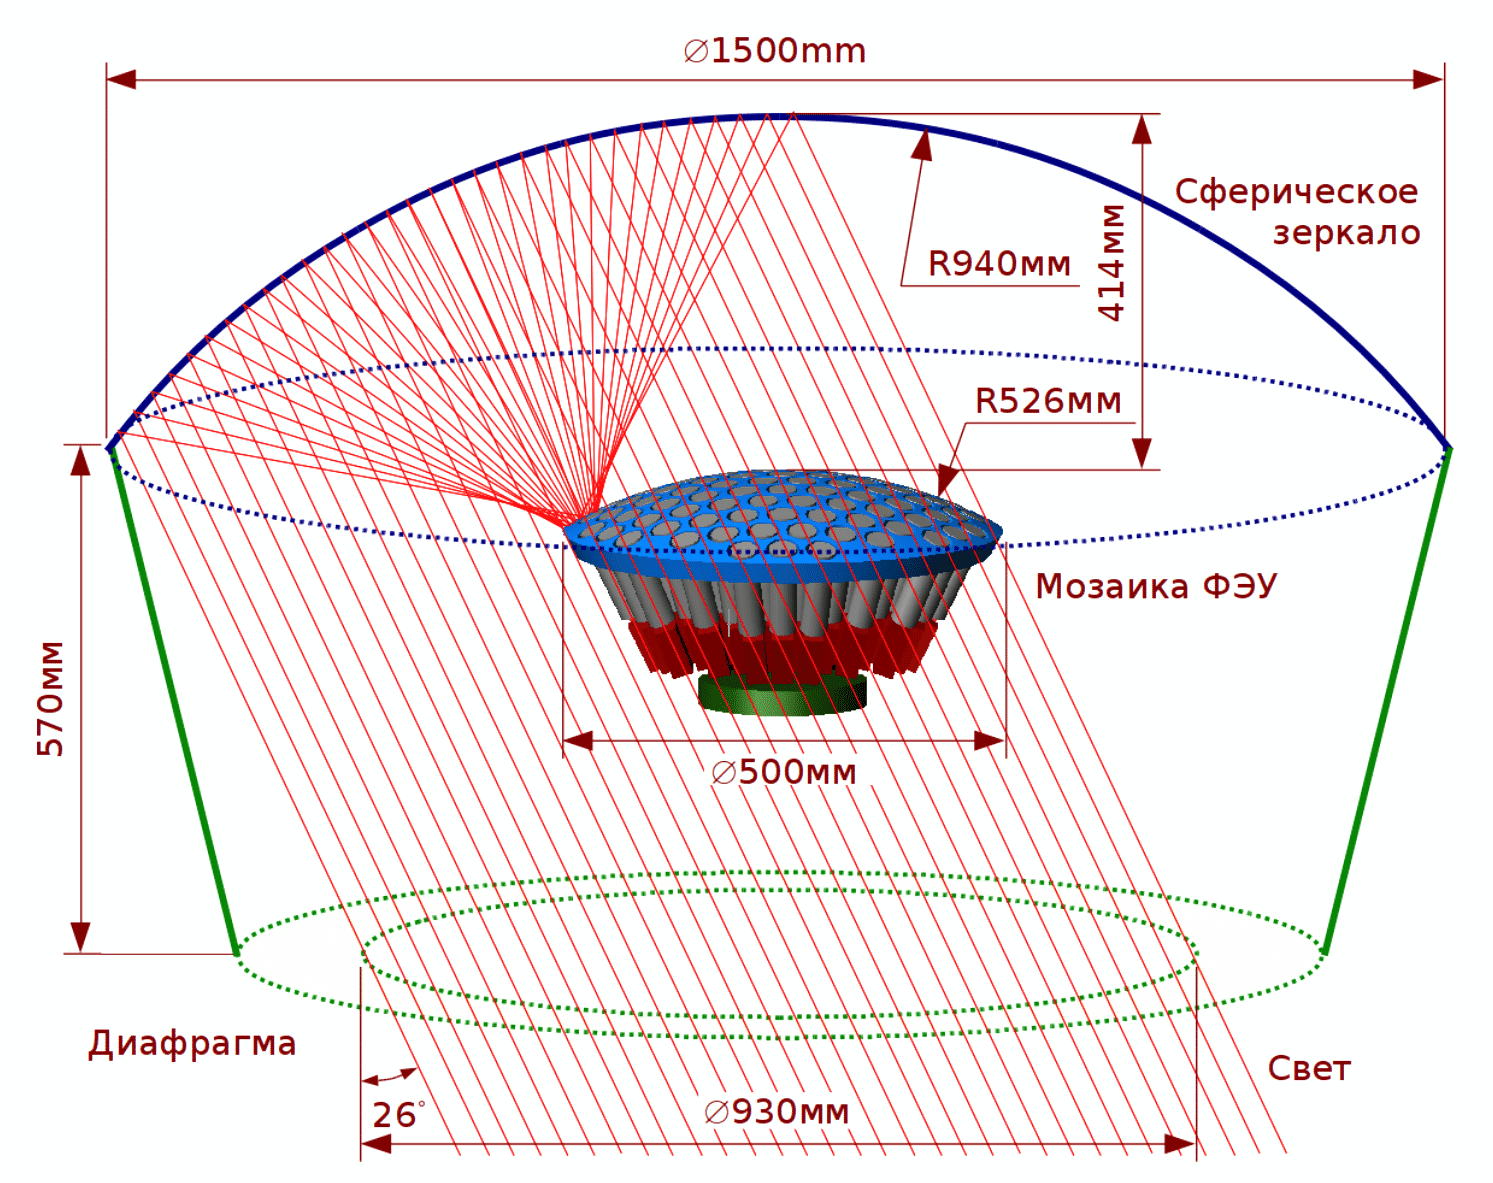
\includegraphics[width=0.9\columnwidth]{optical_scheme}
	\caption{SPHERE-2 detector optical scheme}
	\label{pic:sphere-detector-optical-scheme}
\end{figure}

The PMT mosaic is located near the focal surface of the spherical mirror and consists of 109 PMTs assembled into an approximately hexagonal grid. The center is Hamamatsu R3886, characterized by a larger gain and photocathode area, the rest are Soviet-made PMT 84-3. Hamamatsu was used as a reference PMT during detector calibration \cite{SphereCalibration2016}.

\subsection{Intermediate PMT mode}
\label{sec:photon-to-phels-conversion}

When light hits the PMT photocathode, a photoelectron is emitted with a certain probability. Accelerated by a dynode system, it produces an avalanche of secondary photoelectrons that reach the anode, creating an observable charge. The process of knocking out photoelectrons from the cathode is characterized by the quantum efficiency function, which characterizes the probability with which a photon of a given wavelength will generate a photoelectron in the system.

The electron cascade within a PMT is a fundamentally stochastic process. This is confirmed by direct laboratory measurements of anode charge fluctuations \cite[Fig. 9]{SphereCalibration2016}. If a dynode system has $N \approx 10$ dynodes, and the total electron multiplication factor is $K \approx 10^6$, then the multiplication per dynode will be on average $\sqrt[N]{K} \approx 4$. From this, taking into account some special features of the PMT (the first dynode distinguished by multiplicity, the chance not to hit the dynode at all), one can perform a relatively simple Monte-Carlo to obtain the gain distribution for the PMT84-3, for which laboratory measurements are not available.

The stochastic nature of the PMT amplification is not apparent when measuring high fluxes because of averaging. It is also not important at low fluxes, when the PMT operates in the photon counting mode and individual well-resolved pulses can be observed on the oscillogram. However, in the SPHERE-2 detector PMTs operate in an intermediate mode: the flux is too large for individual photons to be resolved, but not sufficient to achieve effective averaging. This leads to the need for deconvolution problem to be posed in statistical terms.
